% This is samplepaper.tex, a sample chapter demonstrating the
% LLNCS macro package for Springer Computer Science proceedings;
% Version 2.20 of 2017/10/04
%
\documentclass[runningheads]{llncs}
%
\usepackage{graphicx}
% Used for displaying a sample figure. If possible, figure files should
% be included in EPS format.
%
% If you use the hyperref package, please uncomment the following line
% to display URLs in blue roman font according to Springer's eBook style:
% \renewcommand\UrlFont{\color{blue}\rmfamily}

\usepackage{subfig}
\usepackage{multirow}

\begin{document}
%
% \title{Contribution Title\thanks{Supported by organization x.}}
% \title{Knowledge Discovery - Analysis of players data in FIFA 2019}
\title{OZNAL - Dátová analýza dát hráčov z hry FIFA 19}
%
%\titlerunning{Abbreviated paper title}
% If the paper title is too long for the running head, you can set
% an abbreviated paper title here
%
\author{Timotej Zaťko \and Tomáš Hoffer}
%
\authorrunning{T. Zaťko, T. Hoffer}
% First names are abbreviated in the running head.
% If there are more than two authors, 'et al.' is used.
%
\institute{Fakulta informatiky a informačných technológií STU v Bratislave
Ilkovičova 2, 842 16 Bratislava 4\\
\email{xzatkot1@stuba.sk} \email{xhoffer@stuba.sk}\\
\url{https://www.fiit.stuba.sk/}}
%
\maketitle              % typeset the header of the contribution
%
\begin{abstract}
Táto práca obsahuje analýzu dát hráčov z hry FIFA 19, opis dát a ich charakteristiky. V tejto práci skúmame vzťahy atribútov na predikovaný atribút trhovej ceny hráča a jeho hernú pozíciu na ihrisku.

\keywords{Analýza dát, FIFA 19, Strojové Učenie, Regresia, Klasifikácia}
\end{abstract}

\section{Opis problému a motivácia}

Rozhodli sme sa pre analýzu dát hráčov z hry FIFA 19. V hre sa nachádza veľké množstvo hráčov z rôznych krajín, hrajúcich v rôznych súťažiach. Ich schopnosti v hre by mali odzrkadlovať ich schopnosti z reálneho sveta. Tvorcovia hry sa o to snažia vytvorením herných atribútov, akými sú napríklad rýchlosť šprintu, sila strely, zakončovanie alebo hlavičkovanie ktoré dokázali vyjadriť číselne. V projekte sa budeme snažiť na základe týchto atribútov klasifikovať hráčov do hernej pozície a predikovať ich trhovú hodnotu v hre. Keďže hra hráčom neukazuje vždy trhovú hodnotu hráča, ale len jeho atribúty, náš model môže byť užitočný pri určovaní výšky ponúkanej sumy za prestup hráča pri vyjednávaní v hre. Keďže v reálnom svete schopnosti hráčov (napr. zakončovanie) niesú nijako numericky vyjadrené skúsime využiť to, že v hre vyjadrené sú, na zistenie, ktoré atribúty sú dôležité pre určité herné pozície.

\section{Opis dát s charakteristika dát}
 
% TIMO:
 
% - opis dat
% - najskor high level, pocet atributov, pocer kategorickych, pocet numerickych (pred a po predspracovani)
% - spomenut oblasti atributov - skusit ich zadelit do kategorii
%     - hrac ako clovek - meno, narodnost, vyska, hmotnost, vek
%     - hrac ako futbalista - plat, herne atributy (tych je velmi vela - numericke), Work Rate v utoku/defenzivne, pozicia na ihrisku, body type, medzinarodna reputacia, preferovana noha, sila slabsej nohy
%     - hrac a vztah ku klubu - klub, dlzka kontraktu, typ kontraktu, release claause, joined, jersey number
%     - nerelevantne - photo, face...
    
    
% TIMO:
% sekcia ocistenie dat
% - spomenut predspracovanie - ocistenie dat 
%  - konverzie hodnot - financne hodnoty (tisicky, miliony)
%  - konverzie mier - feet to cm, hmotnost
%  - odstranenie znakov. z numerickycha tributov
%  - konverzia dlzky konktraktu (time)

 
Naša dátová sada obsahuje 18207 záznamov - hráčov, ktorý každý z nich má 87 atribútov. Z toho je 42 numerických a 45 kategorických.
 
\subsection{Očistenie dát} \label{ocistenie_dat}
 
Kvôli analýze bolo treba dátovú sadu, očistiť a urobiť predspracovanie niektorých atribútov. Bolo nutné spraviť nasledovné úpravy -- konverzia a očistenie finančných hodnôt (napr. `\$77.5M`, `\$1K`), konverzia mier (napr. `159lbs`, `5'11`), konverzia časových údajov (napr. `Jan 25, 2019`, `2018`) a rozdelenie niektorých atribútov na viac atribútov - niektoré atribúty obsahovali dva numerické atribúty. Taktiež atribút určujúci pozíciu hráča obsahoval až 38 rôznych herných pozícii, preto sme sa rozhodli tento atribút rozšíriť do ďalších dvoch atribútov v ktorých sme podobné pozície spojili čím vznikli dva atribúty s 13 resp. 4 hodnotami. Po týchto úpravách sa nám počet atribútov zmenil na 129 -- 89 numerických a 40 kategorických atribútov.

Toto veľké množstvo atribútov sme zaradili do nasledovných kategórií, uvádzame k nim aj niektoré atribúty. Atribúty sme rozdelili aj na základe toho či jeho hodnotu musela hra nejakým spôsobom odvodiť z reálneho sveta.

\begin{itemize}
\item \textbf{človek} - meno, národnosť, výška, hmotnosť, vek...
\item \textbf{futbalový hráč (reálny svet)} - názov klubu, číslo dresu, dátum príchodu do klubu, dĺžka kontraktu, plat hráča, hosťovský klub, herná pozícia, preferovaná noha
\item \textbf{futbalový hráč (hra)} - trhová hodnota hráča, triky, pracovitosť v útoku/obrane, vhodnosť na určitú špecifickú pozíciu a potenciálny rast (78 atribútov), medzinárodná reputácia
\item \textbf{futbalové schopnosti hráča určené hrou} (celkovo 34 atribútov) - krátke prihrávky, hlavičkovanie, zakončovanie...
\item \textbf{iné atribúty hry} - logo klubu, vlajka (na základe národnosti), typ postavy (tj. typ herného modelu), typ tváre (tj. kvôli herného modelu)
\end{itemize}

\subsection{Analýza chýbajúcich hodnôt} \label{analyza_chybajucich_hodnot}

% TIMO
% - pozreli sme chybajuce hodnoty a vztahy meczi chybajucimi hodnotami
% - ukazat co sme zistili, dat tam ten insight z deepnotu co je, spomenut dendogram

Ako prvé sme sa pozreli na chýbajúce hodnoty v našej dátovej sade. Početnosti sme vizualizovali stĺpcovým diagramom a vzťahy tepelnou mapou a dendrogramom. Zistili sme, že niektorým hráčom chýbajú hodnoty v atribútoch ako sú klub, plat, dĺžka kontraktu, číslo dresu či výkupná klauzula. Tieto hodnoty chýbajú väčšinou spoločne, o čom sme sa presvedčili v dendrograme a tepelnej mape. Je to aj logické, keďže hráč, ktorý nemá klub nemôže poberať plat alebo mať výkupnú klauzulu v kontrakte. Z našich zistení môžeme konštatovať, že ak hráčovi chýbajú hodnoty v atribúte, väčšinou sa nejedná o chybu v úplnosti dátovej sady.

\subsection{Analýza z pohľadu pozície hráča} \label{analyza_z_pohladu_pozicie}

Analýzu sme ďalej realizovali z pohľadu dvoch atribútov, ktoré sa budeme snažiť predikovať - pozíciu hráča (kategorický atribút) a jeho trhovú hodnotu (numerický atribút). Dátová sada celkovo obsahuje 36 herných pozícií. 

Na základe našich futbalových znalostí sme sa rozhodli zoskupiť podobné pozície do skupín, čím sme znížili počet rôznych hodnôt v atribúte `Position` (Fig. \ref{fig:position_grouping}). Môžeme pozorovať, že triedy nie sú vyvážené.

\begin{figure}%
    \centering
    \subfloat[4 herné pozície(`Position (4)`)]{{ 
        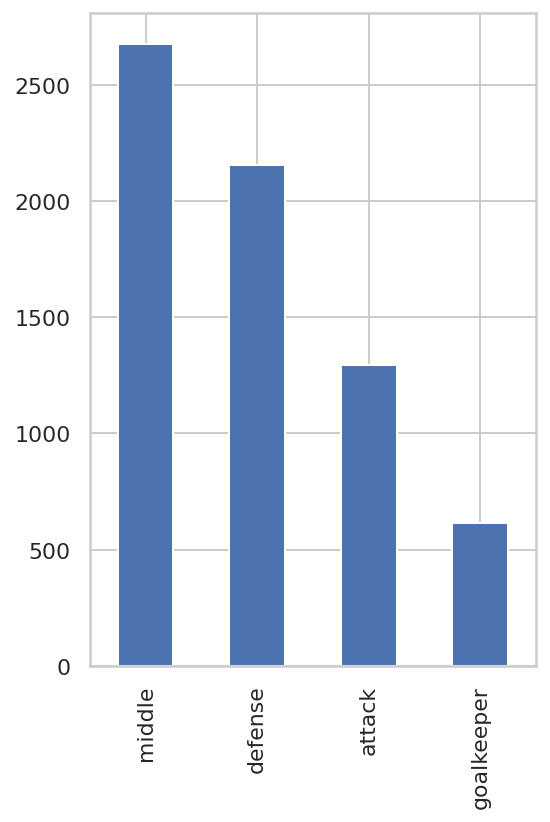
\includegraphics[width=4cm]{images/position_grouping_1}
    }}%
    \qquad
    \subfloat[13 herných pozícií (`Position (13)`)]{{
        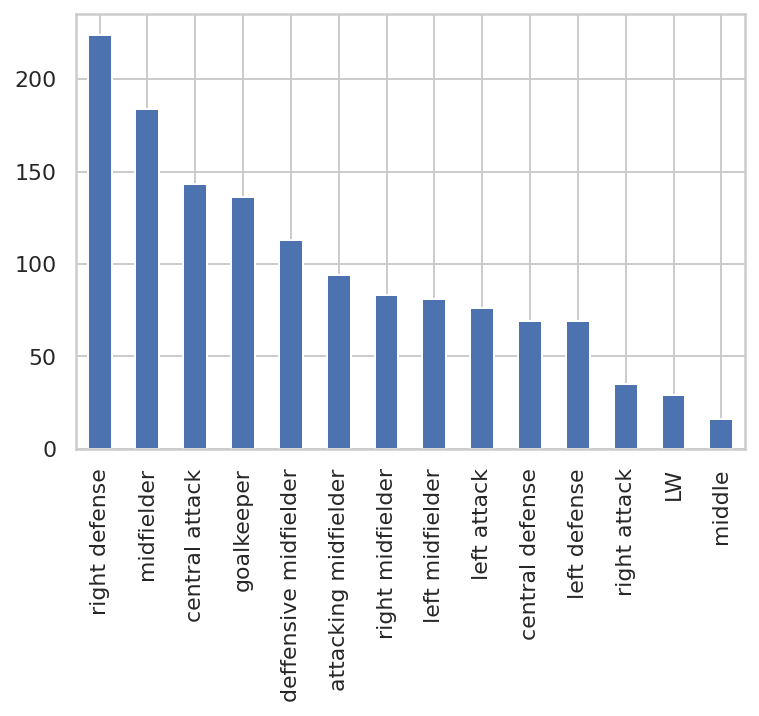
\includegraphics[width=7cm]{images/position_grouping_2}
    }}%
    \caption{Početnosti nových atribútov `Position (4)` a `Position (13)` po zoskupení podobných hodnôt z atribútu `Position`.}%
    \label{fig:position_grouping}%
\end{figure}

Pozíciu sa môžeme pokúsiť predikovať na základe 34 atribútov definujúcich futbalové schopnosti hráča určené hrou. Vizualizovali sme všetky dvojice týchto atribútov a pomocou "scatter plot" -ov  sme hľadali zhluky jednotlivých pozícií. Ako príklad uvádzame vzťah medzi atribútmi `Shot Power` (sila strely) a `Finishing` (zakončovanie), kde môžeme pozorovať jednotlivé zhluky podľa pozície hráča (Fig. \ref{fig:shot_power_finishing_scatter_plot}).

\begin{figure}%
    \centering
    \subfloat[4 herné pozície (`Position (4)`)]{{ 
        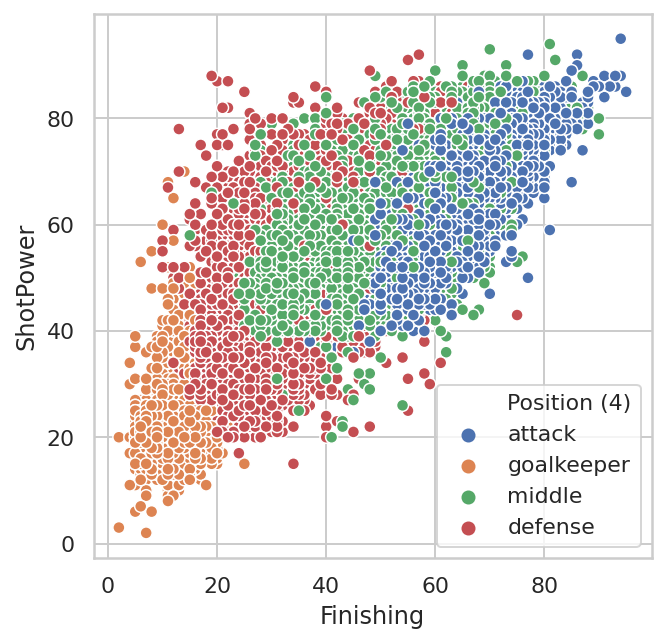
\includegraphics[width=5.5cm]{images/shot_power_finishing_scatter_plot_position_4}
    }}%
    \qquad
    \subfloat[13 henrých pozícií (`Position (13)`)]{{
        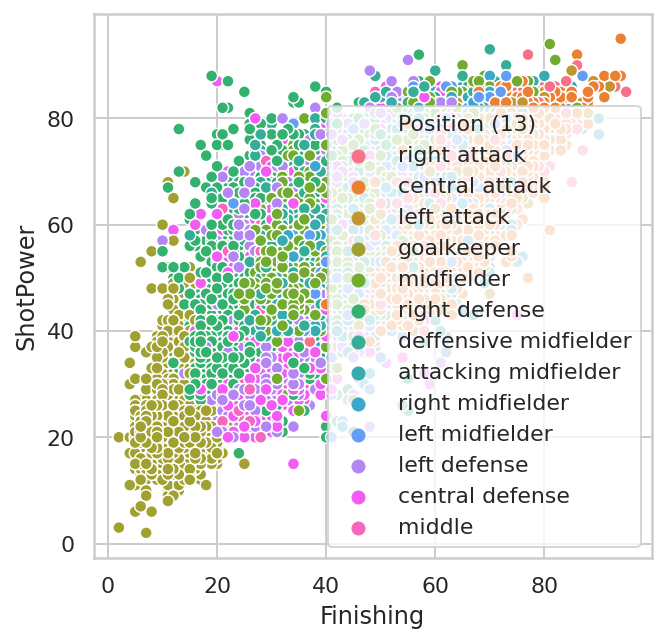
\includegraphics[width=5.5cm]{images/shot_power_finishing_scatter_plot_position_13}
    }}%
    \caption{Vzťah medzi atribútmi `Shot Power` a `Finishing`. Pre 4 herné pozície sú zhluky zreteľnejšie ako pre 13 herných pozícií.}%
    \label{fig:shot_power_finishing_scatter_plot}%
\end{figure}

Z prieskumnej analýzy tiež vyplýva, že pre konkrétne pozície hráčov sú typické určité čísla dresov. Pre brankárov (angl. goalkeeper) je typickým číslom dresu číslo \textit{1} pričom toto číslo nemá priredený žiaden hráč na inej pozícii. Pre útočníkov (angl. attack) to je \textit{9}, pre obrancov (angl. defense) sú to čísla \textit{2 - 6} a pre stredopoloarov \textit{7}, \textit{8} a \textit{10}. Tento atribút môže byť veľmi dobrý na klasifikáciu pozície hráča, avšak my sa v prvom rade zamieriame na predikciu z herných atribútov. Atribúty, ako napríklad čislo dresu nám môžu úlohu príliš zjednodušiť.

Ďaľšou zaujímavosťou je, že v našej dátovej sade sa nachádzajú prevažne hráči ktorí preferujú pravú nohu, avšak na pozícii ľavého obrancu výrazne prevládajú hráči s preferovanou ľavou nohou. (Fig. \ref{fig:preferred_foot_counts}).

\begin{figure}[htp]
    \centering
    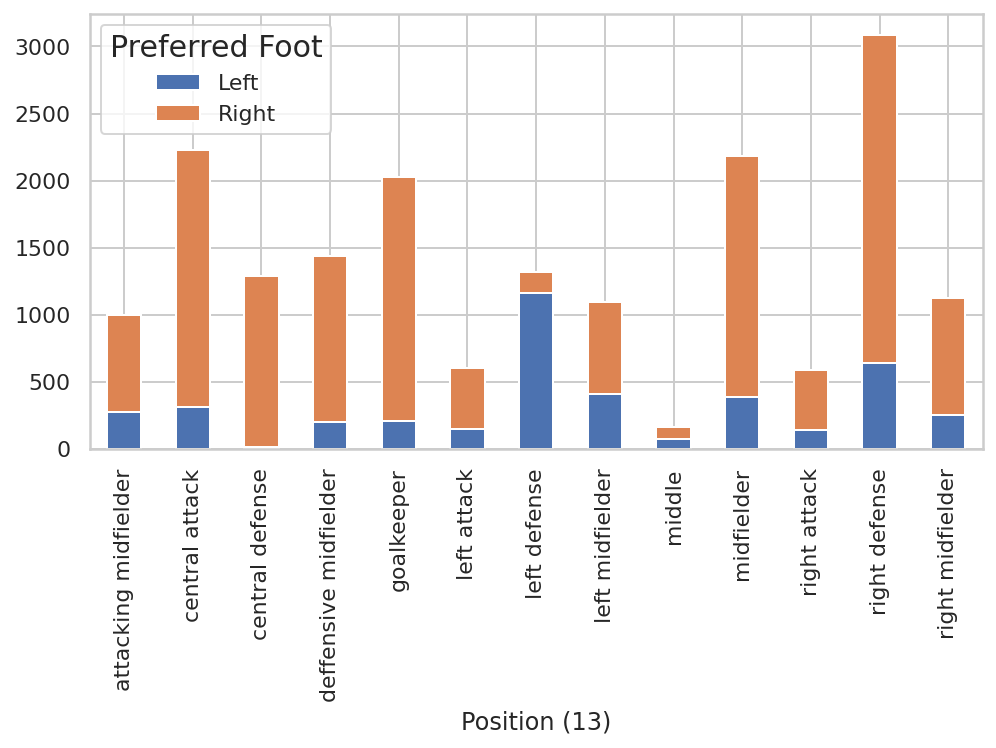
\includegraphics[height=7cm]{images/preferred_foot_counts}
    \caption{Preferovaná noha hráčov podľa hernej pozície.}
    \label{fig:preferred_foot_counts}
\end{figure}

% \begin{figure}[htp]
%     \centering
%     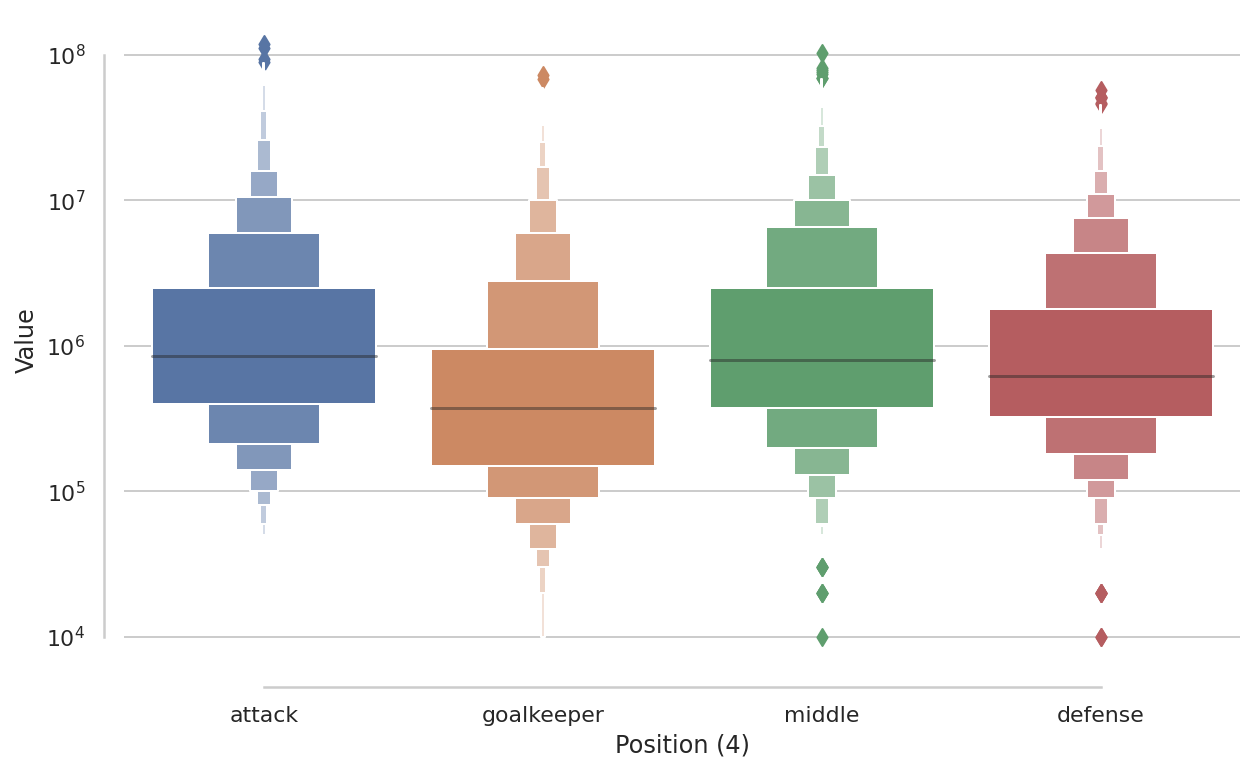
\includegraphics[height=7cm]{images/value_position_boxenplot}
%     \caption{}
%     \label{fig:value_position_boxenplot}
% \end{figure}

\subsection{Analýza z pohľadu trhovej hodnoty hráča} \label{analyza_z_pohladu_trhovej_hodnoty}
Pomocou Pearsonovho korelačného koeficientu sme hľadali korelácie medzi atribútom `Value` a ostatnými numerickými atribútmi. Takmer lineárnu koreláciu (0.99) vykazuje atribút `Release Cause` (Fig. \ref{fig:wage_scatter_plot}). Hráči s vysokou trhovou hodnotou majú v datasete podpísanú zmluvu s vyššou výkupnou klauzulou. Vysokú koreláciu taktiež vykazujú atribúty `Overall` (0.631), `Wage` (0.850) a `International Reputation` (0.656).

\begin{figure}%
    \centering
    \subfloat[Vzťah `Release Cause` voči `Value`.]{{ 
        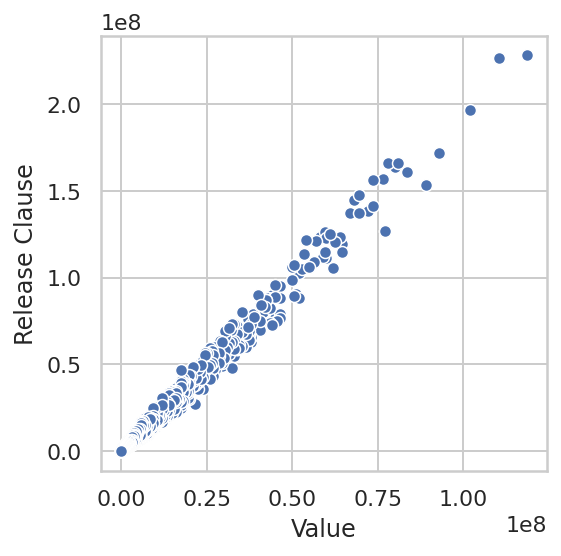
\includegraphics[width=5cm]{images/release_clause_value_scatter_plot}
    }}%
    \qquad
    \subfloat[Vzťah `Wage` voči `Value`.]{{
        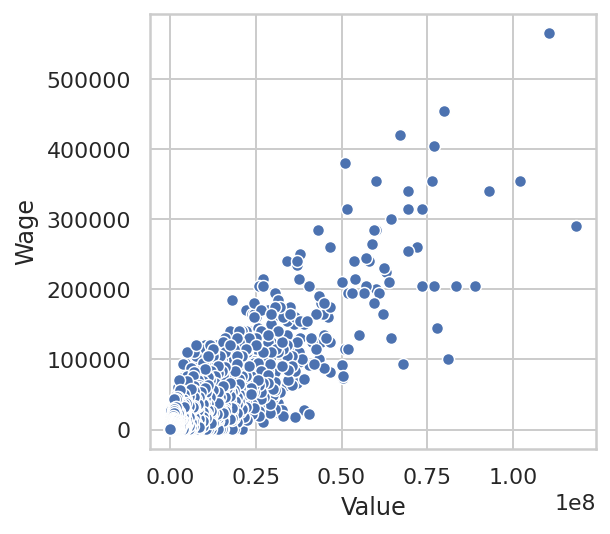
\includegraphics[width=5.5cm]{images/wage_value_scatter_plot}
    }}%
    \caption{Niektoré atribúty vykazujú vysokú mieru korelácie s atribútom `Value`.}%
    \label{fig:wage_scatter_plot}%
\end{figure}


\section{Definovanie úlohy objavovania znalostí}

Rozhodli sme sa, že budeme vykonávať nasledujúce úlohy:
\begin{itemize}
    \item predikcia hernej pozície hráča -- všeobecnej (4 triedy), rozšírenej (13 tried)
    \item predikcia hodnoty hráča (atribút s názvom `Value`)
\end{itemize}

Obe tieto úlohy budeme realizovať z atribútov určujúcich herné shopnosti hráča a následne zo všetkých atribútov. Výsledky porovnáme a očakávame, že model natrénovaný zo všetkých atribútov bude výrazne lepší, keďže niektoré atribúty výrazne ovplyvňujú predikovanú premennú a to -- Release Clause - Value; Jersey Number - Position. 

\section{Predpokladaný scenár riešenia (problémy)}

Predpokladáme, že bude potrebné vykonať nasledovné úlohy:
\begin{itemize}
    \item predspracovanie kategorických hodnôt (tj. one-hot encoding)
    \item normalizácia dát
    \item odstránenie odľahlých pozorovaní
    \item trénovanie modelu
\end{itemize}

Trénovanie modelu zahŕňa výber atribútov (angl. feature selection) a výber a trénovanie modelu. Na úlohu predikcie hodnoty hráča budeme pravdepodobne používať lineárnu regresiu/neurónovú sieť a na určenie hernej pozície hráča rozhodovací strom / náhodný les / SVM / neurónovú sieť.

\section{Predspracovanie dát}
Prvotnému predspracovaniu dát na účely analýzy sme sa venovali v kapitole \ref{ocistenie_dat}
Jedná sa o nasledujúce transformácie dát:
\begin{itemize}
    \item Transformácia hodnôt peňažných atribútov (napr. hodnoty 1.2M, 200K sme transformovali na jednotný numerický tvar)
    \item Dátumové atribúty sme transformovali na jednotný tvar, reprezentovaný UNIX časovou pečiatkou
    \item Atribúty miery (napr. výška a hmotnosť hráča) sme transformovali tak, aby boli v spoločných jednotkách
    \item Špeciálne pozície hráča boli udávané v tvare reťazca \textit{Value+Grow}. Atribúty špeciálnych pozícií sme rozdelili na dvojice aby nám vznikli numerické atribúty.
    \item Atribút \textit{Work Rate} bol udávaný reťazcom v tvare \textit{Attack/Defense}. Tento atribút sme tiež rozdelili na 2 numerické.
    \item Boolean atribúty udávané reťazcami sme transformovali na numerické 0/1
    \item Vytvorili sme 2 nové atribúty Position(4) a Position(13), ktoré reprezentujú pozíciu hráča po zoskúpení pozícií, opísanom v kapitole \ref{analyza_z_pohladu_pozicie}
    \item Vytvorili sme atribút \textit{Contract length}, ktorý reprezentuje dĺžku aktuálne podpísanej zmluvy hráča 
\end{itemize}

Pre účely klasifikačnej a regresnej úlohy sme sa rozhodli kategorické atribúty kódovať pomocou "One-Hot encoding" -u. Numerické atribúty sa nachádzali v rôznych rozsahoch a jednotkách (napríklad hmotnosť v lb, výška v cm, rôzne schopnosti hráča v rozsahu [0,100]). Rozhodli sme sa ich normalizovať na jednotný interval [0,1].

\subsection {Chýbajúce hodnoty}
V kapitole \ref{analyza_chybajucich_hodnot} sme opísali dôvod výskytu chýbajúcich hodnôt. Chýbajúce hodnoty opísané v kapitole \ref{analyza_chybajucich_hodnot} považujeme za opodstatnené a nebudeme ich nahrádzať.

\subsection {Vychýlené hodnoty}
Rozdelenie číselných hodnôt v datasete sme podrobne analyzovali a vyzualizovali. Na základe podrobnej analýzy sme dospeli k záveru, že dataset neobsahuje žiadne vychýlené hodnoty.

\subsection {Problém nevyváženosti tried}
Pri zoskúpení všetkých pozícií do 13 tried sme odhalili nevyváženosť jednotlivých tried (Fig.\ref{fig:position_grouping}), čo by mohlo negatívne ovplyvniť presnosť predikcie. Tento problém sme sa rozhodli riešiť algoritmom SMOTE, ktorý využíva tzv. "oversampling" a vytvára syntetické inštancie minoritnej triedy pomocou lineárnej kombinácie reálnych inštancií.\cite{AlbertoFernandez2018}

\section{Výber atribútov}
Predikciu pri oboch typoch úloh sa budeme snažiť realizovať pomocou 34 atribútov definujúcich futbalové schopnosti hráča určené hrou. Využijeme tiež demografické údaje, napr. výšku, hmotnosť a vek. K tejto základnej množine atribútov sme sa dopracovali na základe doménovej znalosti a rozsiahlej prieskumnej analýzy. V častiach \ref{analyza_z_pohladu_pozicie} a \ref{analyza_z_pohladu_trhovej_hodnoty} sa venujeme výberu týchto atribútov a opisujeme dôvody, prečo sme niektoré atribúty do tejto množiny nezahrnuli.
V druhej etape riešenia vyskúšame úlohy predikcie realizovať s využitím všetkých atribútov a úspešnosti modelov porovnáme. Očakávame mierny nárast úspešnosti pri použití všetkých atribútov.

Pri riešení klasifikačnej úlohy rozšírime základnú sadu atribútov o atribúty \textit{Preferred Foot}, \textit{Work Rate Attack} a \textit{Work Rate Defense}. 
Pri regresnej úlohe využijeme dopočítaný atribút \textit{Contract Length} a tiež medzinárodnú reputáciu hráča.

\section{Výber metrík pre evaluáciu úspešnosti TODO}
\section{Predikcia pozície hráča (klasifikácia)}

Úlohu sme sa v prvej etape rozhodli riešiť pomocou viacerých jednoduchých modelov. Klasifikácia hráča do 4 pozícií už pri základných nastaveniach modelov vykazovala vysokú úspešnosť. V nasledujúcej tabuľke uvádzame modely a ich úspešnosti pri predikcii pozície. Ako metriku sme sa rozhodli sledovať f1 skóre.
\begin{table}[]
    \centering
    \begin{tabular}{|l|l|l|l|l|}
    \hline
    \multirow{2}{*}{model} & \multicolumn{4}{l|}{f1-skóre (pozícia)} \\ \cline{2-5} 
     & attack & defense & goalkeeper & middle \\ \hline
    Rozhodovací strom & 0,74 & 0,86 & 1,0 & 0,76 \\ \hline
    \begin{tabular}[c]{@{}l@{}}Logistická regresia\\ (10-násobná krížová validácia)\end{tabular} & 0,82 & 0,93 & 1,0 & 0,86 \\ \hline
    Metóda podporných vektorov & 0,80 & 0,93 & 1,0 & 0,85 \\ \hline
    \end{tabular}
    \caption{\label{tab:f1_position4}Úspešnosti jednoduchých modelov pri predikcii 4 tried pozície}
    \end{table}

    \begin{figure}[htp]
        \centering
        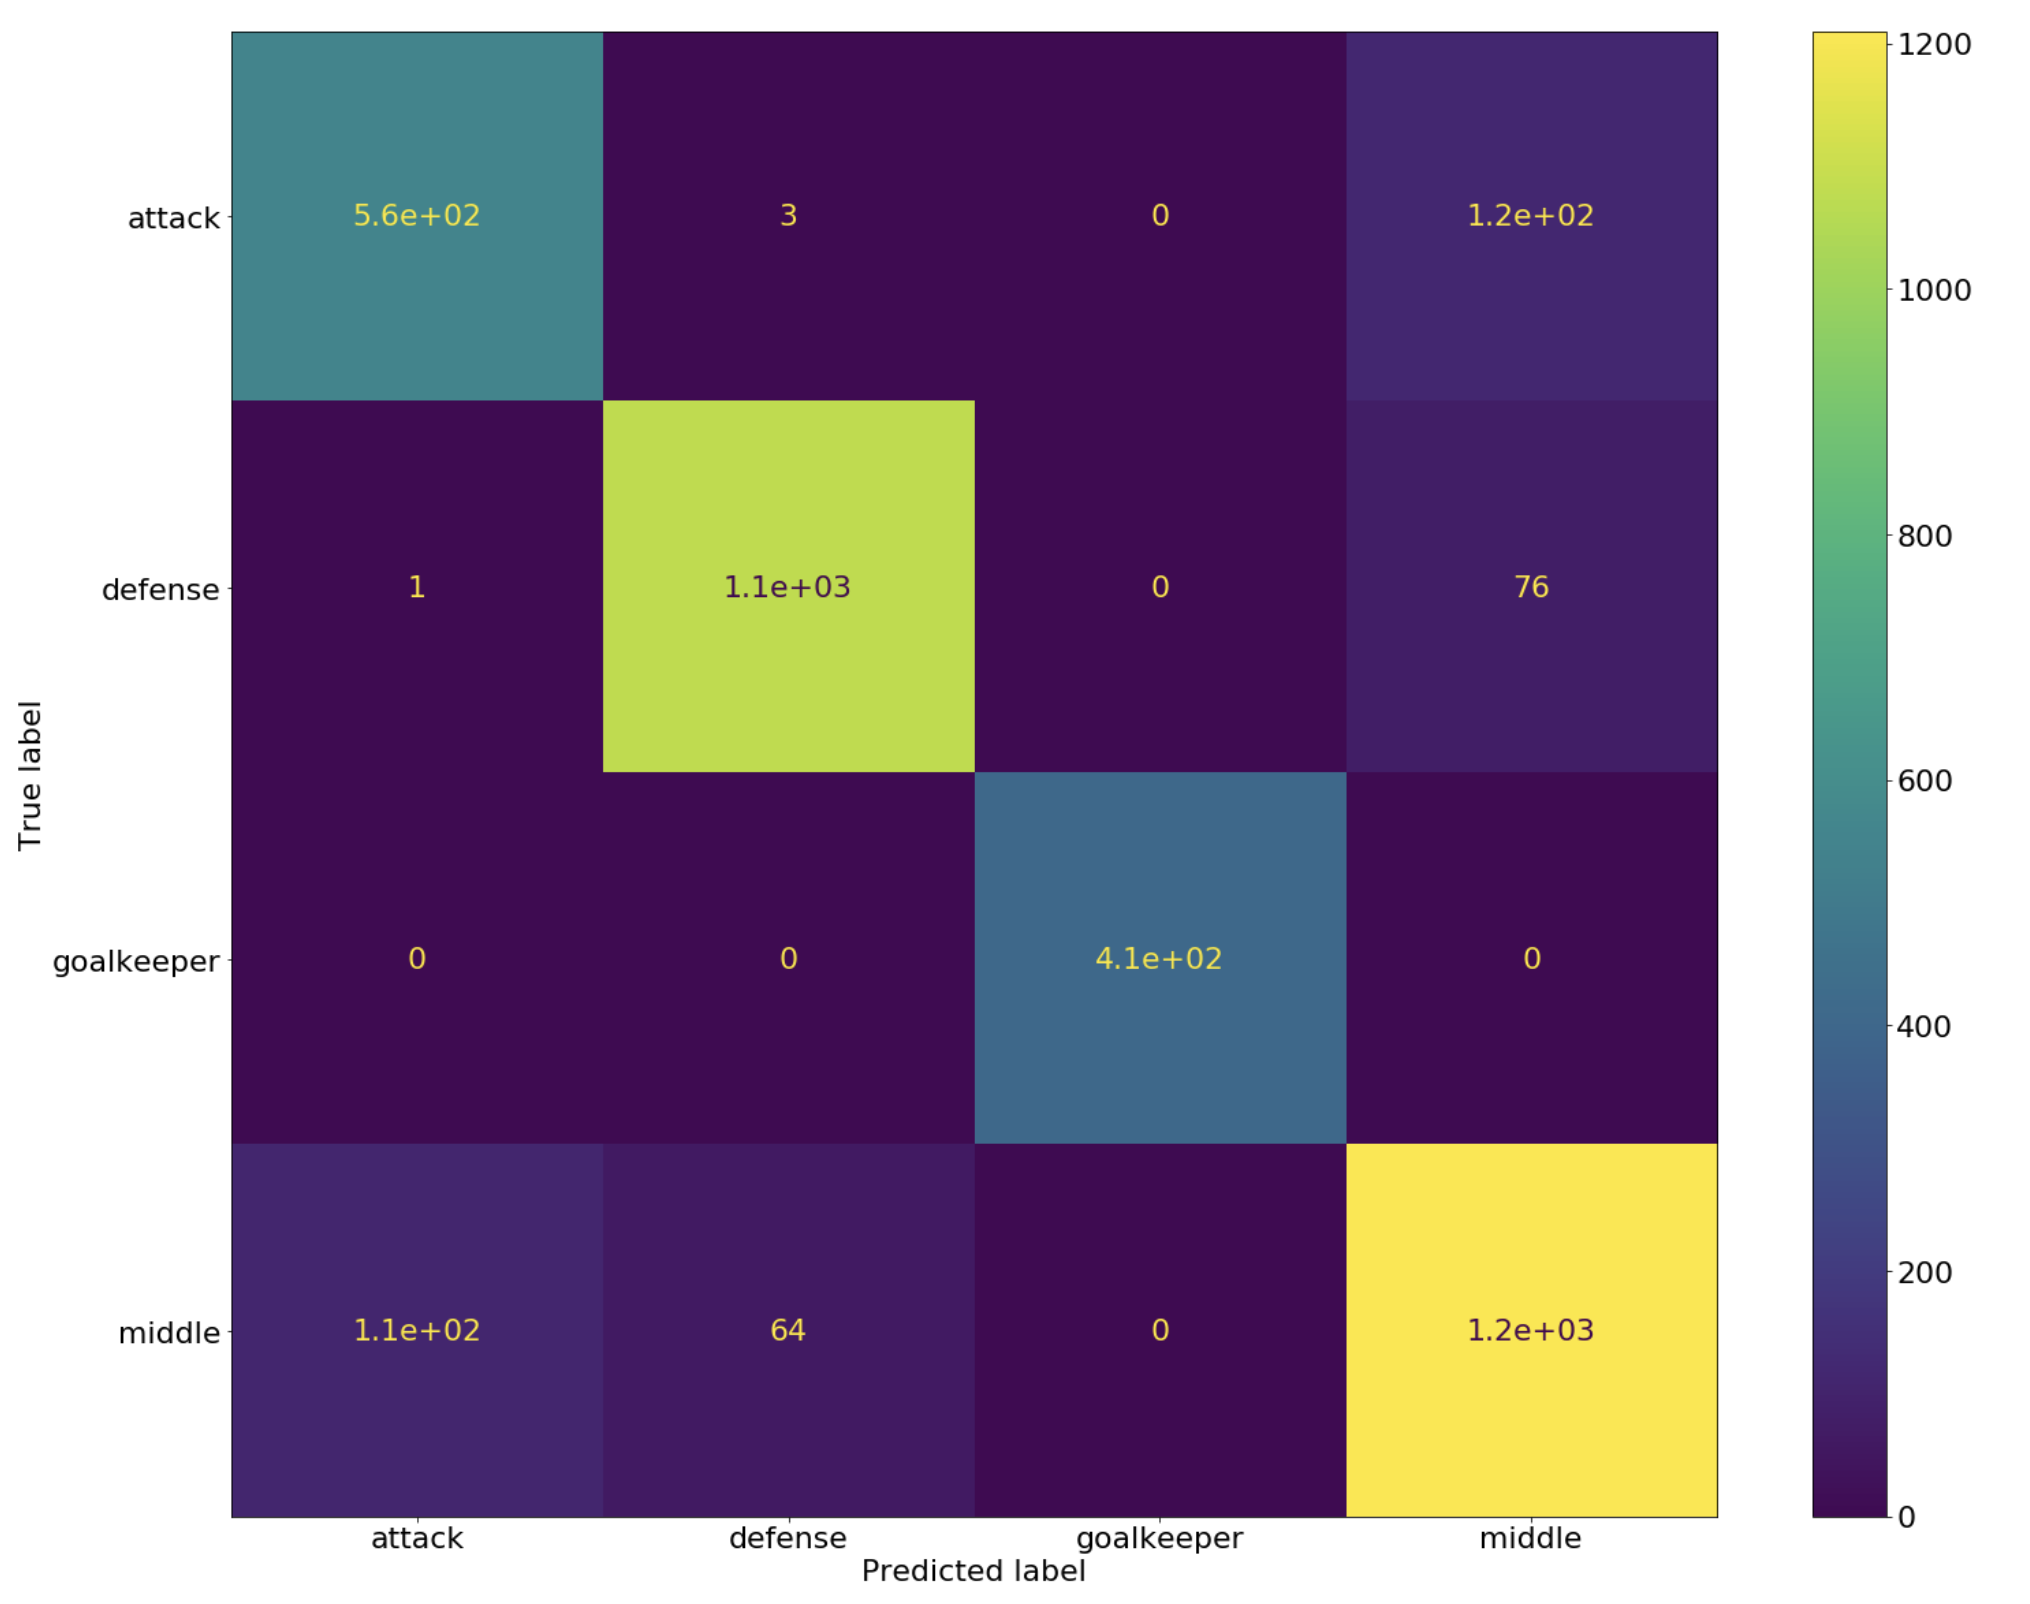
\includegraphics[height=10cm]{images/confusion_matrix_position4_logicticCV}
        \caption{Chybová matica pre logistickú regresiu (4 pozície).}
        \label{fig:confusion_4}
    \end{figure}

Pri klasifikácii do 13 tried pozície je úspešnosť jednoduchých modelov významne nišia. F1-skóre je pre niektoré pozície vysoké (right defense = 0,92) ale niektoré pozície model vôbec nepredikoval (middle = 0,0) 
Úlohu budeme ďalej riešiť pomocou neurónových sietí. 

\begin{figure}[htp]
    \centering
    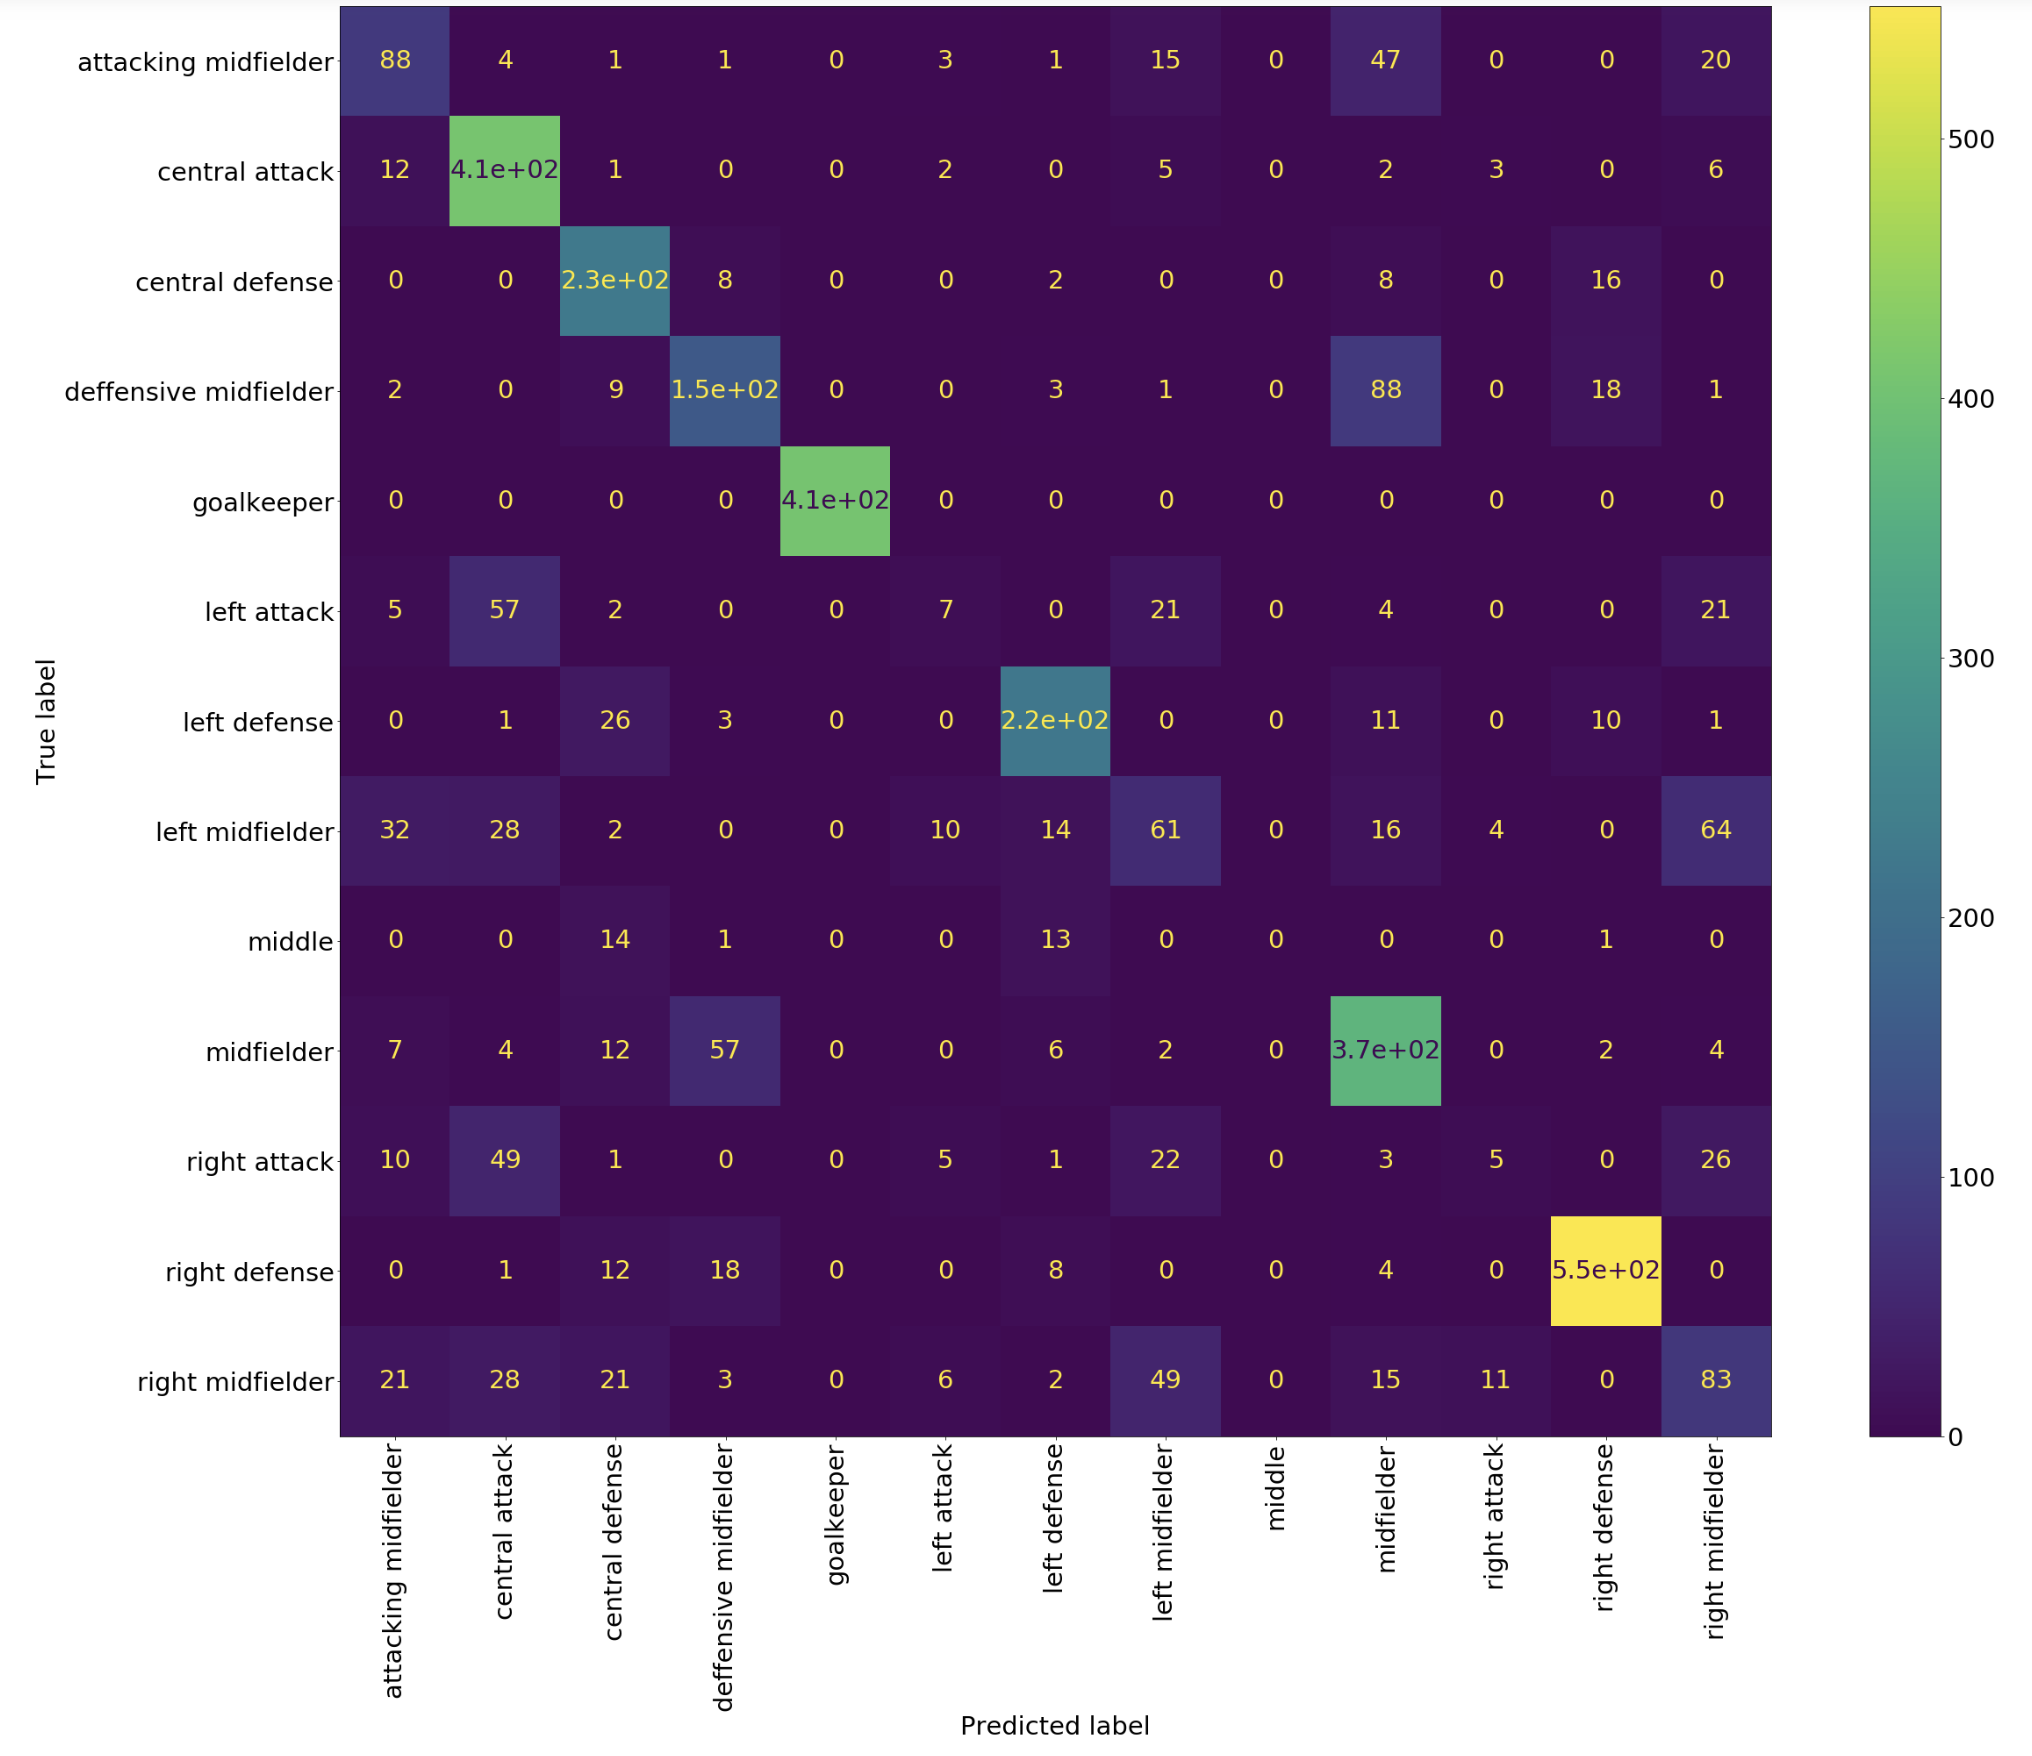
\includegraphics[height=10cm]{images/confusion_matrix_position13_logisticCV}
    \caption{Chybová matica pre logistickú regresiu (13 pozícií).}
    \label{fig:confusion_4}
\end{figure}



\section{Predikcia trhovej hodnoty hráča (regresia)}


\section{Existujúce práce TODO dokoncit}
Soto-Valero, C. na klasifikáciu pozície hráča do štyroch tried v rovnakom datasete najprv využil PCA na extrakciu čŕt a redukciu dimenzionality. Následne využil zhlukovanie na klasifikáciu hráčov do 4 pozícií a pomocou "gradient tree boosting" algoritmu ohodnotil dôležitosť jendotlivých atribútov. Medzi najdôležitejšie atribúty na predukciu patria "dribbling", "standing tackle" a "goalkeeper reflexes". \cite{RICYDE1165}

\bibliographystyle{splncs04}
\bibliography{references}


\end{document}
